\section{Descrição das técnicas implementadas para a solução, principalmente do classificador}

O grande objetivo deste trabalho foi o desenvolvimento de um software capaz de 
determinar a qual das quatro classes \emph{BI-RADS} uma imagem de exame de mamografia 
pertence. Para este fim, o funcionamento do software é dividido em duas grandes 
etapas: a de obtenção e pré-processamento dos dados e a de treinamento.

\newpage
\subsection{Obtenção dos dados e Pré-processamento}

\begin{figure}
    \centering
    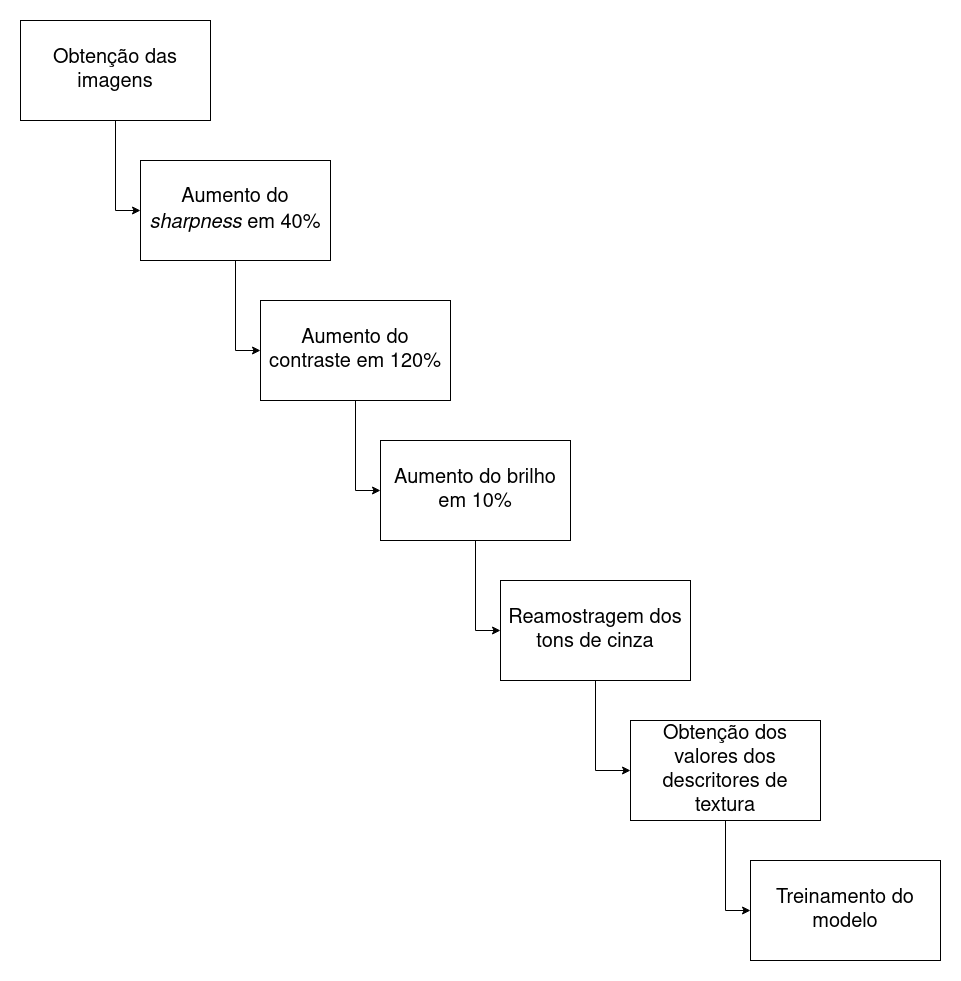
\includegraphics[scale=0.3]{Imagens/Fluxograma.png}
    \caption{Fluxograma das etapas antes do treinamento do classificador}
\end{figure}

Como ilustrado na figura 1, a primeira etapa consiste na obtenção das imagens.
Nessa etapa as imagens são separadas de forma aleatória entre um conjunto de 
treino e um conjunto de teste, mas ainda mantendo um balanceamento equivalente 
entre as classes \emph{BI-RADS} de acordo com a porcentagem estipulada para treinamento.

A etapa de pré-processamento das imagens foi identificada como imperativa e de 
extrema relevância para o treinamento do modelo. Essa etapa tem como objetivo 
realçar características de cada imagem em ambos conjuntos de treino e teste a 
fim de aumentar a discrepância entre as imagens de classes diferentes,  e assim 
obter um classificador com maior acurácia. Primeiro é utilizada a biblioteca 
\emph{Pillow} para realçar o \emph{sharpness} das imagens em 40\% a fim de realçar mais as 
bordas e regiões limítrofes nas imagens. Após isso é feito um aumento de 120\% 
no contraste da imagem a fim de alterar as tonalidades de cinza e realçar mais 
as diferenças de cores entre os pixels. Por fim, é feito um aumento do brilho em 10\%. 
Para a etapa de pré-processamento também foi explorada a possibilidade da 
implementação de um filtro de suavização gaussiana, mas os testes rapidamente 
demonstraram que a resolução das imagens se mostrou muito baixa, e a implementação 
da suavização gaussiana suprimiu grande partes das sutilezas e detalhes finos das imagens.
O filtro de utilização gaussiano pode ser habilitado no menu de opções avançadas da
interface, mas por padrão ele está desabilitado. O grupo recomenda a sua utilização
apenas em imagens que tenham resolução superior a 128x128 pixels. 

Também é feita uma reamostragem dos tons de cinza da imagem de acordo com o valor 
definido pelo usuário na interface. Esta reamostragem é feita após a escolha pelo 
usuário de um valor entre 1 e 32 tons de cinza, e também é implementada com a biblioteca 
\emph{Pillow}. Após isto, são calculadas as matrizes de co-ocorrência circulares C1, C2, C4, C8 e C16 
da imagem já pré-processada e obtidos os descritores de textura para cada uma delas. 
Finalmente, os valores obtidos para os descritores de textura das imagens no conjunto 
de treinamento são alimentados ao modelo de identificação como parte da etapa de treinamento.

\subsection{Treinamento}

A fim de obter um modelo de alta acurácia, foi utilizado o \emph{Support Vector Machine} (\emph{SVM}) 
com kernel linear e parâmetro de regularização (C) com valor 1.4. Tendo em vista as imagens 
que foram fornecidas e que compõem o dataset entende-se que a escolha de utilizar \emph{SVM} é 
mais relevante à medida que foi identificada uma variação intra-classe relativamente alta 
nas imagens, e esta variação poderia facilmente afetar de forma negativa um modelo baseado 
em redes neurais. Outro grande motivador foi a preocupação na sensibilidade do classificador
em relação a outliers. Após diversos testes, a kernel linear se mostrou resistente a 
outliers no conjunto de treinamento e apresentou os melhores resultados nas métricas de 
acurácia e especificidade, o que o configurou como a escolha ideal.

Para a etapa de treinamento, primeiro o classificador é criado com uma kernel linear e 
parâmetro de regularização com valor 1.4. Após isso, o classificador é alimentado com 
os valores dos descritores de textura obtidos de cada imagem no conjunto de dados de 
treinamento, bem como a categoria à qual esse grupo de descritores pertence. Após esse ponto, 
o classificador já é considerado treinado e está pronto para identificar a qual classe \emph{BI-RADS}
as imagens no conjunto de teste pertencem. Também foi implementada uma função de classificação 
de uma única imagem, que pode ser escolhida individualmente pelo usuário. 